\documentclass[12pt,fleqn]{article}
\usepackage{graphicx, array, subfig}

\title{\bf Nature-inspired Methods for Solving the Mobile Subscriber Equipment Problem}

\author{Matthew Saltz \\
        The University of Georgia \\
        Athens, Georgia 30602 U.S.A.}

\date{2013 April 21}

\begin{document}
\maketitle
\section{Introduction}
This paper details the results of different methods for solving the problem of optimally purchasing
mobile subscriber equipment for battlefield communications network configurations.  
The two methods used are nature-inspired, with one being a genetic algorithm and the 
other using particle swarm optimization.  Because the search space is large, these
heuristic techniques are necessary if these tools are to be used in a real-time setting;
for example, as part of a software for tutoring future field agents.  
\section{Experimentation}    
The input to the algorithms is the number of DNVTs and the number of MSRTs required to be supported. We tested each method on three different DNVT/MSRT combinations. To judge the fitness of a result, we ensure that no item purchased lies outside the quantity constraints for that item, and we penalize purchases that yield more functionality than necessary.  We also, of course, measure the degree to which a given configuration of purchases can support the inputs. We ran each of the
algorithms 1000 times, and measured the percentage of times that each obtained the result with the maximum fitness (relative to its other results). We call this measure {\em repeatability}. Each algorithm gave the same output for each input pair, which increases our confidence in our results. These outputs are shown in Figure~\ref{fig:configs}. It can be seen in Figure~\ref{fig:repeatability} that the repeatability of both methods is very high, with both approaching 100\%. The PSO algorithm, however, took much longer to achieve the same level of accuracy (though it is possible that these runtimes could be improved upon).  Due to the fact that the algorithms agree with each other, these repeatabilities seem
to indicate that the algorithms are reliable in finding optimal or close to optimal results. Specific purchasing orders given by the algorithms are shown for several different DNVT/MSRT pairs in Figure~\ref{fig:configs}. 

\begin{figure}
{\small
\begin{center}
\begin{tabular}{ | l | l !{\vrule width 2pt} l | l | l | l | l | l | l !{\vrule width 2pt} l |}
\hline
MSRT & DNVT & NC & LEN & SEN-1 & SEN-2 & SCC & RAU & NAI & Fitness \\ \hline
672 & 1495  & 9  & 0   & 33    & 11    & 1   & 27  & 0   & 327.36  \\ \hline 
200 & 1000  & 5  & 0   & 23    & 7     & 1   & 8   & 0   & 520.62  \\ \hline
700 & 50    & 4  & 0   & 3     & 1     & 1   & 28  & 0   & 140.78  \\ \hline
\end{tabular}
\end{center}
}
\caption{Resulting configurations and fitnesses obtained by both the GA and the PSO algorithm}
\label{fig:configs}
\end{figure}

\begin{figure}
{\tiny
\hspace{-2.5em}
%\begin{center}
\begin{tabular}{ | l | l !{\vrule width 2pt} l | l | l | l | l | l | l !{\vrule width 2pt} l |}
\hline
MSRT & DNVT & GA Repeatability (\%) & PSO Repeatability (\%) & GA Average Runtime (s) & PSO Average Runtime (s)\\ \hline
672 & 1495  & 100                   & 100                   & 3.15                    & 23.43                  \\ \hline 
200 & 1000  & 99.6                  & 100                    & 3.65                   & 14.92                  \\ \hline
700 & 50    & 99.8                  & 100                    & 4.49                   & 12.98                  \\ \hline
\end{tabular}
%\end{center}
}
\caption{Repeatabilities and Runtimes for GA and PSO}
\label{fig:repeatability}
\end{figure}

\begin{figure}[h]
  \centering
  \subfloat[]{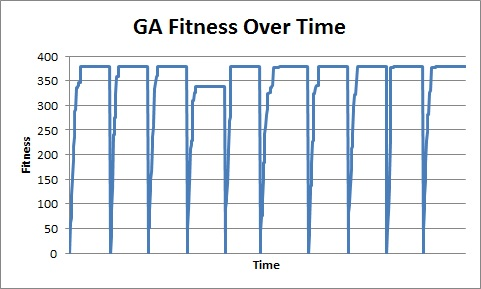
\includegraphics[width=0.9\textwidth]{./ga_fitness}}\\
  \subfloat[]{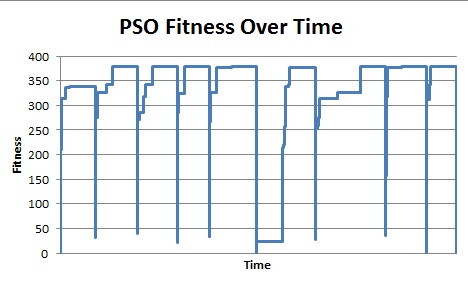
\includegraphics[width=0.9\textwidth]{./pso_fitness}}
  \caption{Each trial run consisted of 10 actual iterations of the algorithm,
           and the best individual from any iteration was chosen as the result 
           of that run.} 
\end{figure}

\end{document}

